\documentclass{beamer}
\usepackage{amsmath} %pour tous les trucs de math
\usepackage{systeme} %pour tous les systemes d'équations
%\usepackage{ bbold }  %pour toutes les doubles lettres
\usepackage{ dsfont } % le 1 en double
\usepackage{amssymb}  %pour les double Lettres
\usepackage{IEEEtrantools} %pour les équations en collonnes
\usepackage{amsthm} %pour les preuves
\usepackage[english]{babel} % la langue utilisée
\usepackage[utf8]{inputenc} % encodage symboles entrée
\usepackage[T1]{fontenc} % encodage symboles sortie
\usepackage{fancyhdr} %pour les entêtes et pied de page
%\usepackage[math]{blindtext} % pour le Lorem ipsum
%\usepackage{enumitem} %pour changer les listes
\usepackage{caption}
\usepackage{subcaption}

\usetheme{Madrid}

\DeclareMathOperator*{\argmin}{argmin}
\DeclareMathOperator*{\argmax}{argmax}
\DeclareMathOperator*{\row}{row}
\DeclareMathOperator*{\col}{col}
\DeclareMathOperator*{\divergence}{div}
\DeclareMathOperator*{\vect}{vect}
\newcommand{\dd}{\emph{d}}
\newcommand{\R}{\mathbb{R}}
\newcommand{\N}{\mathbb{N}}
\newcommand{\Z}{\mathbb{Z}}
\newcommand{\C}{\mathbb{C}}
\newcommand{\T}{\mathbb{T}}
\newcommand{\un}{\mathds{1}}
\newcommand{\ie}{i.e.\;}
\newcommand{\None}{\text{None}}
\newcommand{\com}[1]{\textcolor{ForestGreen}{[~\emph{#1}~]}}
\newcommand{\ps}[2]{\langle#1,#2\rangle}

%Information to be included in the title page:
\title{Computational Optimal Transport:\\ A Comparison of Three Algorithms}
\author{Benoît Müller}
\institute{intermediate presentation}
\date{2023}

\begin{document}

\frame{\titlepage}

\begin{frame}
    \frametitle{Framework}
    \begin{itemize}
    \item Monge problem
    $$(MP) = \inf_{T_{\#}\mu=\nu} \int c(x,T(x)) d\mu(x)$$
    in this project, the cost is $c(x,y)=\|x-y\|^2$
    
    Theorical garantee:
    \begin{alertblock}{Brenier's theorem}
    Let $\mu$ and $\nu$ be measures on $\R^d$ with finite second moments $\int\|x\|^2d\mu$,$\int\|x\|^2d\nu$, and such that $\mu$ is absolutely continuous w.r.t. the Lebesgue measure.
    
    Then Monge problem is uniquely attained at an optimal transport map $T$ and $T=\nabla\phi$ for a convex map $\phi$.
    \end{alertblock}
    \item Gradient of convex function is actually necessary and sufficient.
    \end{itemize}
\end{frame}

\begin{frame}
    \frametitle{Discretization leads to a linear program}
    \begin{itemize}
    \item Discretize $$\mu = 1/n\sum^n_{i=1} \delta_{x_i},\quad\nu = 1/n\sum^n_{j=1} \delta_{y_j}$$
    $$C_{ij} = \|x_i-y_j\|^2$$
    \item I prove the steps to derive this lemma:
    \begin{alertblock}{Lemma for discrete formulation}
    The discretization leads to a linear program 
    $$(MP) 
    = \min_{\substack{P\in\{0,1\}^{n\times n} \\ P\un=\un=P^\top\un}} \ps{P}{C}  
    = \max_{\substack{u,v\in\R^n \\ u_i+v_j\leq C_{ij}}} \ps{\un}{(u+v)}$$
    called linear sum assignment problem (LSAP).
    \end{alertblock}
    \end{itemize}
\end{frame}

\begin{frame}  
    \frametitle{Discretization leads to a linear program (II)}
    \begin{itemize}
    \item (LSAP) can be solved with the Hungarian algorithm, a primal-dual by using the sufficient and neccessary KKT conditions:
    \begin{equation*}
    \begin{cases}
    P \geq 0,\quad P\un = P^\top\un = \un & \text{: primal feasibility} \text{ (pf)}  \\
    u_i + v_j \leq C_{ij}  & \text{: dual feasibility}  \text{ (df)} \\
    P_{ij}(C_{ij} - u_i - v_j) = 0  &\text{: complementary slackness} \text{ (cs)}
    \end{cases}
    \end{equation*}
    \item First polynomial time algorithm for (LSAP), recognized as the predescessor of primal-dual algorithm
    \item The algorithm as unvariants during the process: (df) and (cs) remain true and (pf) partially true:  $P \geq 0,\quad P\un \leq \un \geq P^\top$
    %\item Filling $P$ where $C_{ij} = u_i + v_j$ is equivalent to finding a matching on subgraph. Done by growing augmenting tree.
    %\item When filling fail to continue, change dual variable to add new possibilities.
    \item Solve a matching problem indepependent of costs at each iteration.
    \end{itemize}
\end{frame}

\begin{frame}{Hungarian algorithm}
    \begin{itemize}
        \item Representation of variables
        \begin{itemize}
            \item Sets represented by Boolean arrays.
            \item Permutation matrix $P$ represented by its permutation map as an array.
        \end{itemize}
        \item Takes an arbitrary cost and tolerance , return a solution such that KKT holds with tolerance. 
        \item If cost values are integers, convergence in finite amount of time $O(n^3)$ is assured.
        If scalars, we can either use the tolerance, or approximate them by rationals and re-scale them to integers.
        
        ––> Seem to be a better solution, no theoretical guarantee to stop with scalars and tolerance.
    \end{itemize}
\end{frame}
\begin{frame}{Hungarian algorithm: numerical results}
\begin{figure}
    \centering
    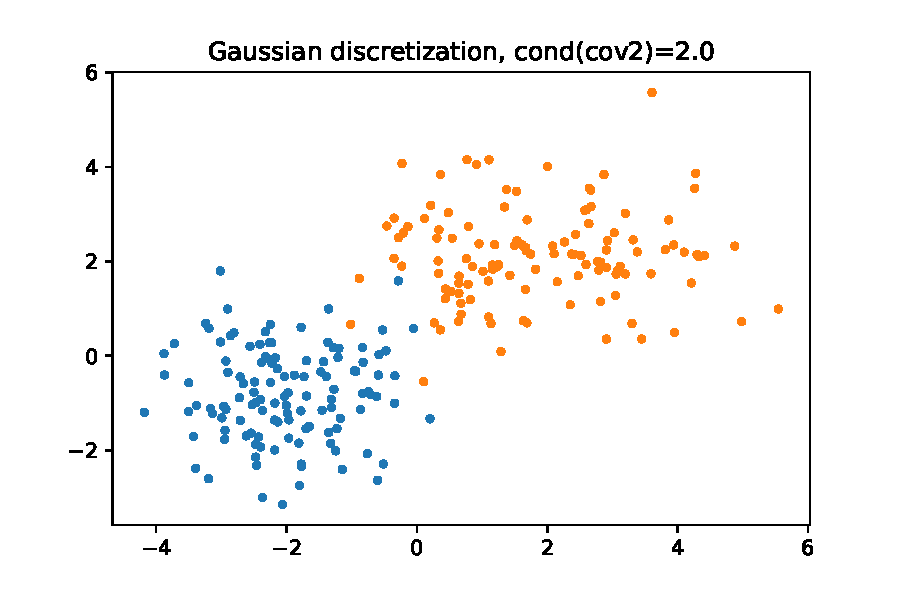
\includegraphics[width=0.8\textwidth]{graphics/hungarian_mu_nu.pdf}
    \caption{source and target density}
    \label{fig:nu}
\end{figure}
\end{frame}
\begin{frame}{Hungarian algorithm: numerical results}
\begin{figure}
    \centering
    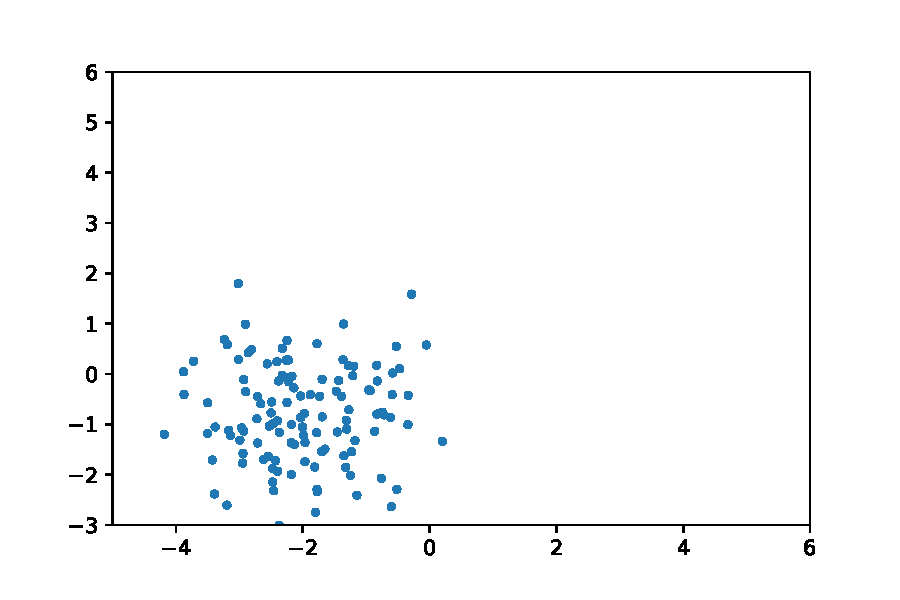
\includegraphics[width=0.8\textwidth]{graphics/hungarian_geodesic0.pdf}
    \caption{geodesic}
    \label{fig:nu}
\end{figure}
\end{frame}
\begin{frame}{Hungarian algorithm: numerical results}
\begin{figure}
    \centering
    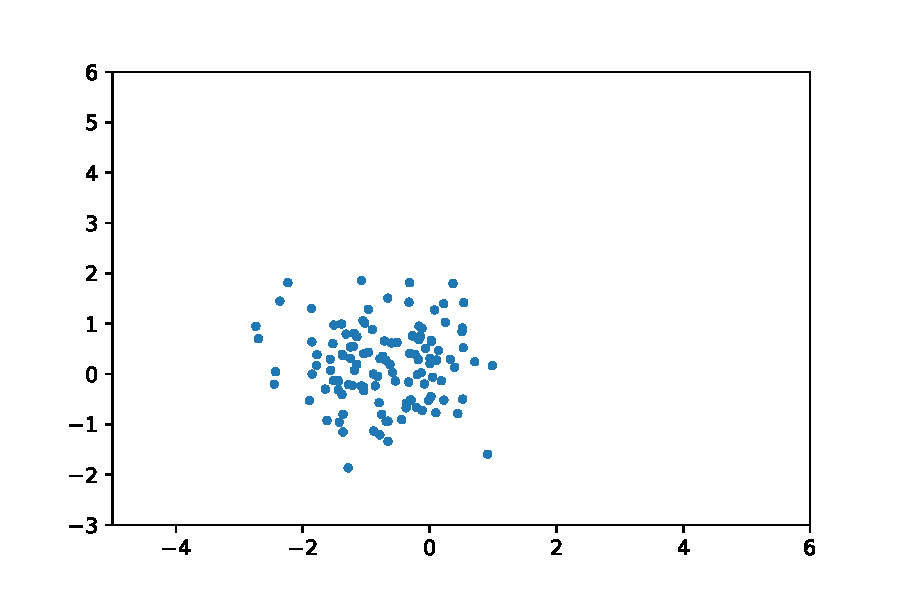
\includegraphics[width=0.8\textwidth]{graphics/hungarian_geodesic1.pdf}
    \caption{geodesic}
    \label{fig:nu}
\end{figure}
\end{frame}
\begin{frame}{Hungarian algorithm: numerical results}
\begin{figure}
    \centering
    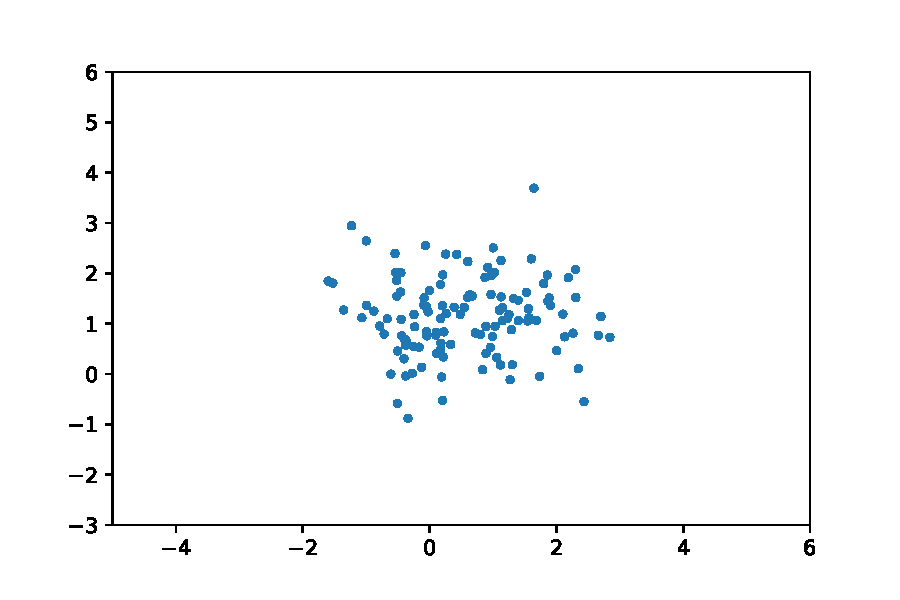
\includegraphics[width=0.8\textwidth]{graphics/hungarian_geodesic2.pdf}
    \caption{geodesic}
    \label{fig:nu}
\end{figure}
\end{frame}
\begin{frame}{Hungarian algorithm: numerical results}
\begin{figure}
    \centering
    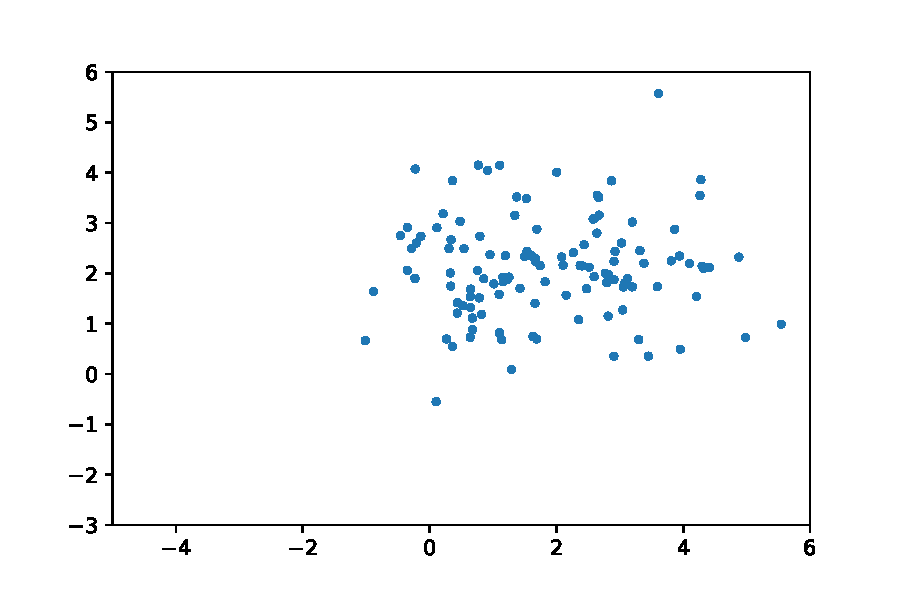
\includegraphics[width=0.8\textwidth]{graphics/hungarian_geodesic3.pdf}
    \caption{geodesic}
    \label{fig:nu}
\end{figure}
\end{frame}
\begin{frame}{Hungarian algorithm: numerical results}
\begin{figure}
    \centering
    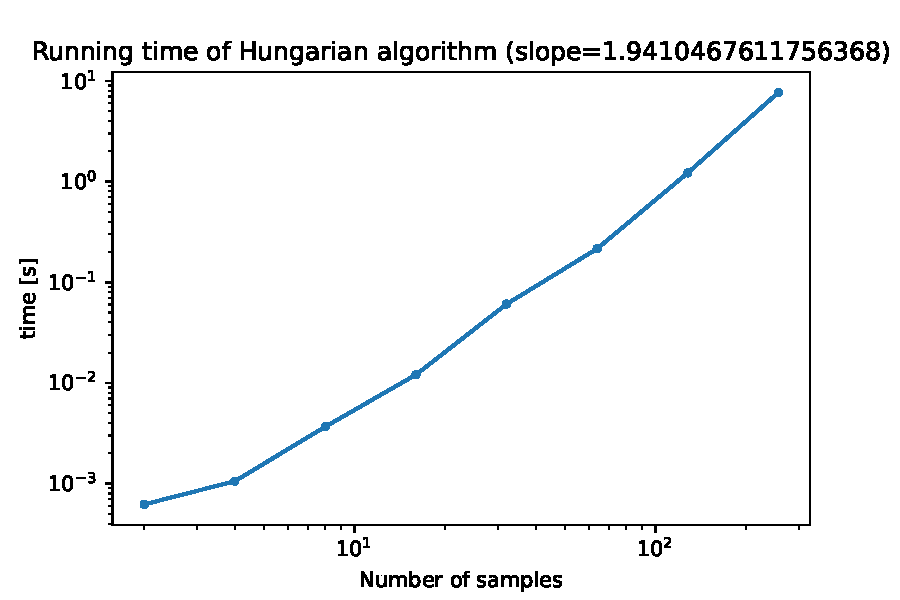
\includegraphics[width=0.8\textwidth]{graphics/hungarian_time.pdf}
    \caption{Error}
    \label{fig:nu}
\end{figure}
\end{frame}
\begin{frame}{Hungarian algorithm: numerical results}
\begin{figure}
    \centering
    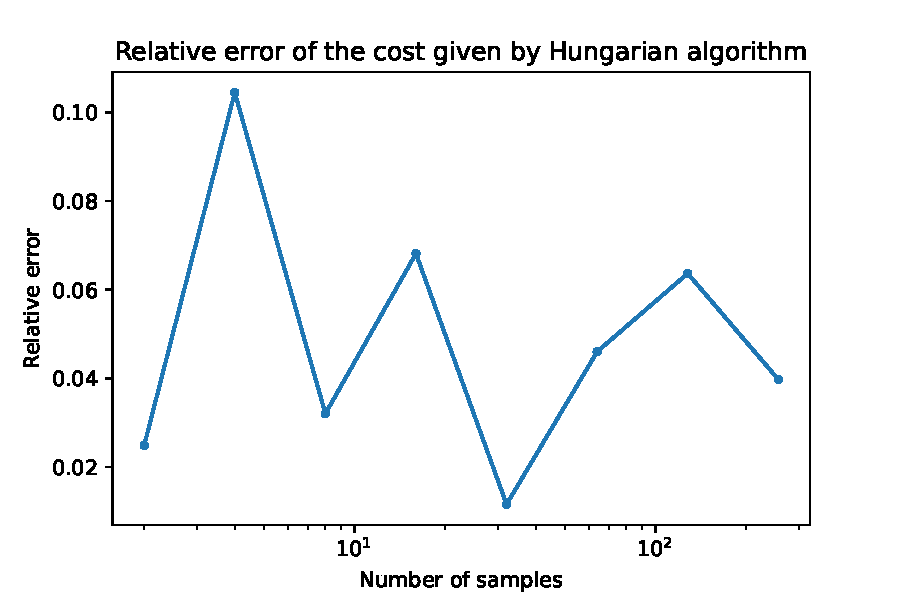
\includegraphics[width=0.8\textwidth]{graphics/hungarian_error.pdf}
    \caption{Error}
    \label{fig:nu}
\end{figure}
\end{frame}

\begin{frame}{Dynamical formulation: Benamou-Brenier}
    \begin{itemize}
        \item change the view of optimal transport to a Riemanian interpretation.
        \item For a optimal transport map $T$, $T_t=(t-1)Id + tT$ induce a geodesic $\rho_t = T_{t\#}\mu$ in the Wasserstein space.
        \item Search for $\rho_t$ among curves of measures instead of searching for $T$.
        \item Characterization of $\rho_t$: suppose it is a density, and $T_t$ is a flow of a vector field $v_t$:
        $$\partial_t T_t = v_t(T_t)$$
        $$T_0 =Id, T_1=T.$$
        Then we can derive the continuity equation $$\partial_t\rho_t + div(\rho_tv_t) = 0$$
        which formulate the continuity of the curve and the mass conservation.
        \end{itemize}
\end{frame}

\begin{frame}{Dynamical formulation: Benamou-Brenier (II)}
    \begin{itemize}
        \item among all curves, the geodesic corresponding to the optimal transport is the one that minimize the following kinetic energy:
        \begin{alertblock}{Lemma for dynamic formulation}
        $$(MP) = \inf \bigg\{ \int\rho\|v\|^2 \;\bigg|\; \partial_t\rho_t + div(\rho_tv_t) = 0 ,\, \rho_0=\mu,\, \rho_1=\nu \bigg\} $$
        \end{alertblock}
        \item Massage the formula:
        \begin{itemize}
        \item Change of variable 
        $(\rho,v)\mapsto(\rho ,\rho v)=:(\rho,m)$ make the objective function convex.
        \item Use Lagrange multiplier $\phi$ to include the constraints
        \item writing the convex integrand $\|m\|^2/m$ as a suppremum of affine functions indexed by a parabolic set $K$.
        \end{itemize}
        \end{itemize}
        \end{frame}
        
\begin{frame}{Dynamical formulation: Benamou-Brenier (III)}
    \begin{itemize}
       \item We can manage to rewrite the problem as
        $$\sup_{M}\inf_{\phi,q} \big(\iota_K(q) + G(\phi) +\ps{M}{\nabla_{t,x}\phi-q}_{L^2}\big)$$
        where
        \begin{itemize}
           \item $M=(\rho,m)$,
           \item $\phi:[0,1]\times\R^d\to\R$ is a well chosen test function,
           \item $q:[0,1]\times\R^d\to\R^{d+1}$,
           \item $G$ is the linear map 
           $G(\phi) = \int\phi(0,.)\rho_0-\phi(1,.)\rho_1$,
           \item $\iota_K$ is $\infty$ on $K$, and 0 else. 
       \end{itemize}
       \item This saddle problem can be seen as a reversed Lagrangian for $\phi,q$ with $M$ as a dual variable with constraint $\nabla_{t,x}\phi=q$
       \item Solve the augmented Lagrangian that has the same saddle points:
       $$ L_r(M,\phi,q) = F(q) + G(\phi) +\ps{M}{\nabla_{t,x}\phi-q} + \frac{r}{2}\|\nabla_{t,x}\phi-q\|^2$$
    \end{itemize}
\end{frame}

\begin{frame}{Dynamical formulation: Benamou-Brenier (IV)}
    The problem $\sup_{M}\inf_{\phi,q} L_r(M,\phi,q)$ is solved with a modified Uzama algorithm:
    \begin{itemize}
       \item $\phi_{k+1} = \min_\phi L_r(M_k,\phi,q_k) $ 
       \item $q_{k+1} = \min_q L_r(M_k,\phi_{k+1},q)$
       \item $M_{k+1} = M_{k} + r(\nabla_{t,x}\phi_{k+1}-q_{k+1})$
    \end{itemize}
    It leads to three subproblems:
    \begin{itemize}
        \item Solve a Poisson equation with Neumann conditions \\ –> "Poisson step"
        \item  Project points to the parabola K \\ –> "Projection step"
        \item –> "Dual step"
    \end{itemize}
\end{frame}

\begin{frame}{Poisson step}
\begin{itemize}
    \item The poisson equation looks like this:\\ $-r\Delta_{t,x}\phi = \divergence_{t,x}(M-rq)$ \\
    $r\partial_t\phi(0,.) = \rho_0 - \rho(0,.) + ra(0,.)$\\
    $r\partial_t\phi(1,.) = \rho_1 - \rho(1,.) + ra(1,.)$
    \item The boundary of $[0,1]\times\R^d$ is $\{0,1\}\times\R^d$, with normal derivative $\pm\partial_t$.
    \begin{itemize}
    \item Problem well posed up to a constant.
    \item Space $[0,1]\times\R^d$ infinite. 
    \end{itemize}
    \item We can work in a finite space by considering the hyper-torus $\T=[0,1]\times(\R^d/\Z^d)$
    \begin{itemize}
        \item $[0,1]^{d+1}$ as a space-time
        \item With space periodic boundary conditions
        \item The cost becomes 
        $c(x,y) = \sum_i\min\{(x_i-y_i)^2,\,1-(x_i-y_i)^2\}$
        \item Problem well posed up to a constant.
    \end{itemize}
\end{itemize}
\end{frame}

\begin{frame}{Poisson step: numerical computation}
Choice of solver, finite differences on a regular grid and sparse linear solver.\\
For an equation $\Delta u = f$ on $\Omega$, $\partial_t u=g$ on $\Gamma_N$, the finite differences are:
\begin{itemize}
    \item Second derivative: centered 3 point stencil $$D_i^2U = h^{-2}(U_{i-1}-2U_i+U_{i+1})$$
    \item How to manage boundary terms:
    \begin{itemize}
        \item Space boundary (periodic): $U_0:=U_N$, $U_{N+1}:=U_1$ \\
        Represented by the $(N-1)\times (N-1)$ matrix:
        $$ A_P = 
        h^{-2}\begin{bmatrix}
            -2 & 1 &  & 1 \\
            1 & \ddots & \ddots &  \\
             & \ddots & \ddots & 1 \\
            1 &  & 1 & -2 
        \end{bmatrix}  $$
        with system $A_P (U_1,\dots,U_{N-1})^\top = (F_1,\dots,F_{N-1})^\top$
    \end{itemize}
\end{itemize}
\end{frame}

\begin{frame}{Poisson step: numerical computation (II)}
\begin{itemize}
    \item \dots boundary terms
    \begin{itemize}
        \item Time boundary with Neumann condition: use of ghost points $U_0$ and $U_{N+1}$ and $O(h^2)$ centered differences on $U_1$ and $U_N$. 
        $$D_1^2U = h^{-2}(U_{0}-2U_1+U_{2}) + O(h^2)$$
        $$DU_1 = (2h)^{-1}(U_{2}-U_0) + O(h^2)$$
        Similar for $U_N$, eliminate the ghost points and get a $N\times N$ representation matrix:
        $$ A_N = h^{-2}\begin{bmatrix}
               -2 & 2  &    &   & \\
                1 & -2 & 1  &   & \\
                  & \ddots  & \ddots & \ddots & \\
                  &    & 1  & -2 & 1  \\
                  &    &    & 2 & -2
            \end{bmatrix}  $$
            with system $$A_N (U_1,\dots,U_{N-1})^\top = (F_1+2h^{-1}G_1,F_2,\dots,F_{N-2},F_{N-1}-2h^{-1}G_N)^\top$$
    \end{itemize}

\end{itemize}
\end{frame}

\begin{frame}{Poisson step: numerical computation (II)}
    \begin{itemize}
    \item 
    In 2D space, we have a 3D(space-time) Poisson equation, and the matrix of the linear system associated to the vectorization
    $$ A = I_{N-1}\otimes I_{N-1}\otimes A_N 
    + I_{N-1}\otimes A_P\otimes I_N  
    + A_P\otimes I_{N-1}\otimes I_N$$
    we get the equation
    $$ A\vect(U) = vect(\tilde{F})   $$
    \item 
    The solution is unique up to constant: $\ker(A) = span(\un)$.
    \begin{itemize}
        \item $(A^\top,\un)^\top$ gives a well defined linear system but is not square anymore.
        \item $
        \begin{bmatrix}
            A & \un \\
            \un^\top & 0  
        \end{bmatrix}  $
         is invertible and gives a solution for a selected mass (even if $\tilde{F}$ isn't exactly orthogonal to $\un$ as it should).
         \item Solve system with a sparse solver, either direct methods (sparse Cholesky: scipy.sparse.linalg.spsolve) or iterative (MINRES).
    \end{itemize}
    \end{itemize}
    \end{frame}

\begin{frame}{Poisson step: numerical computation (II)}
    \begin{itemize}
    \item Projection on $K=\bigl\{(a,b):\R\times\R^d\to\R\times\R^d \,\big|\, a + \|b\|^2/2\leq0 \text{ pointwise}\bigl\}$
    \item The set K is the revolution of a parabola: rewrite it as a 2D problem.
    \item Implementation find a root of the 3-degree polynomial resulting of the orthogonality equations
    \begin{itemize}
        \item Newton method, converges in approx 20 steps.
        \item Analytic solution using Cardano's formula, faster.
    \end{itemize}
    \end{itemize}
\end{frame}

\begin{frame}{Benamou-Brenier method}
\begin{itemize}
    \item Used object oriented programming
    \item A class representing the problem, and keep track of the variables used multiple times such as the Laplacian matrix.
    \item Step done by internal methods that update the object, possibility to display evolution or plot the result.
    \item Projection step and dual step have linear complexity. Poisson step determine the complexity since it is heavier because of the linear problem to solve. Sparse solver use heuristic to reorder the dimensions, but should be $O(N^2)$.

\end{itemize}
\end{frame}

\begin{frame}{Dynamic formulation: numerical results}
\begin{figure}
    \centering
    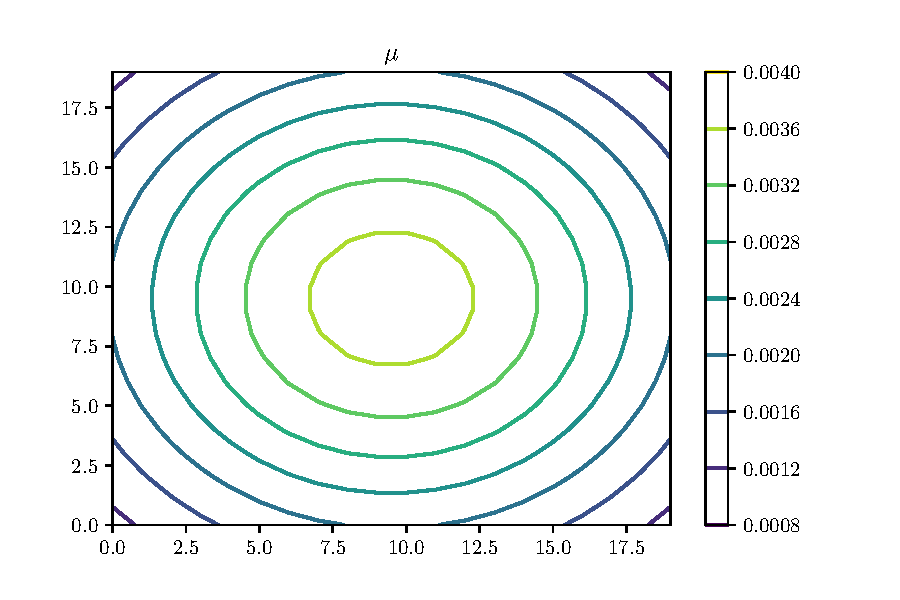
\includegraphics[width=0.8\textwidth]{graphics/mu.pdf}
    \caption{initial density}
    \label{fig:mu}
\end{figure}
\end{frame}
\begin{frame}{Dynamic formulation: numerical results}
\begin{figure}
    \centering
    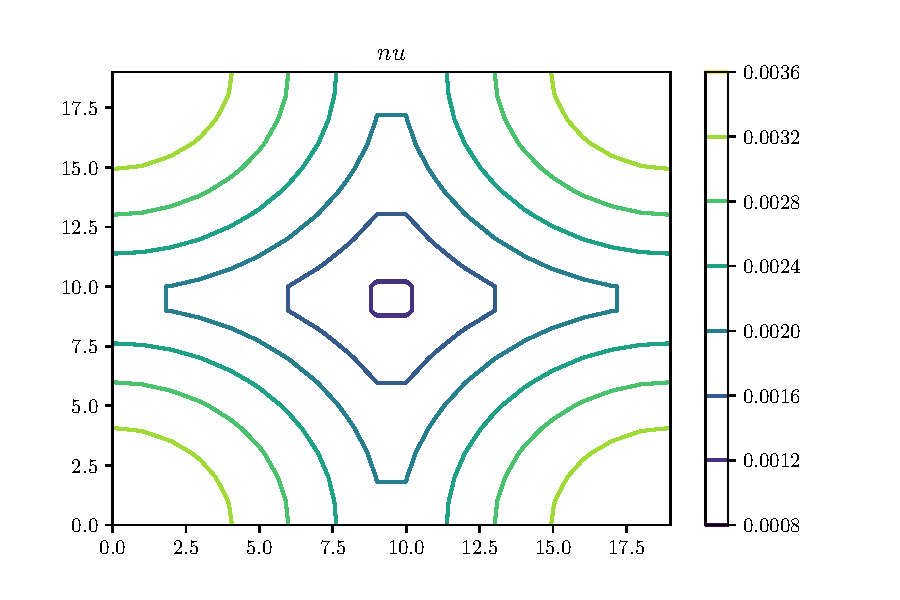
\includegraphics[width=0.8\textwidth]{graphics/nu.pdf}
    \caption{target density}
    \label{fig:nu}
\end{figure}
\end{frame}
\begin{frame}{Dynamic formulation: numerical results}
\begin{figure}
    \centering
    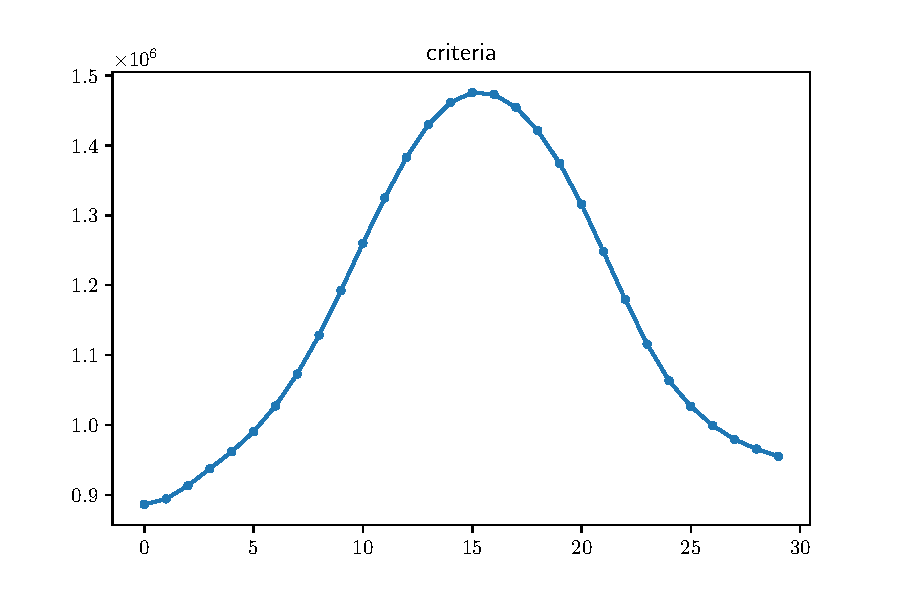
\includegraphics[width=0.8\textwidth]{graphics/criteria.pdf}
    \caption{criteria}
    \label{fig:nu}
\end{figure}
\end{frame}
\begin{frame}{Dynamic formulation: numerical results}
\begin{figure}
    \centering
    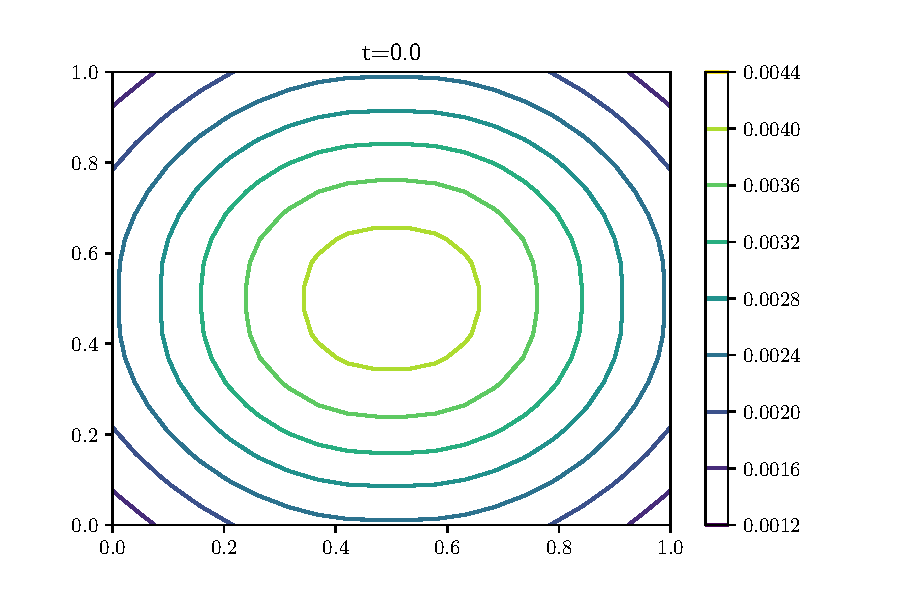
\includegraphics[width=0.8\textwidth]{graphics/rho(0).pdf}
    \caption{rho(t)}
    \label{fig:nu}
\end{figure}
\end{frame}
\begin{frame}{Dynamic formulation: numerical results}
\begin{figure}
    \centering
    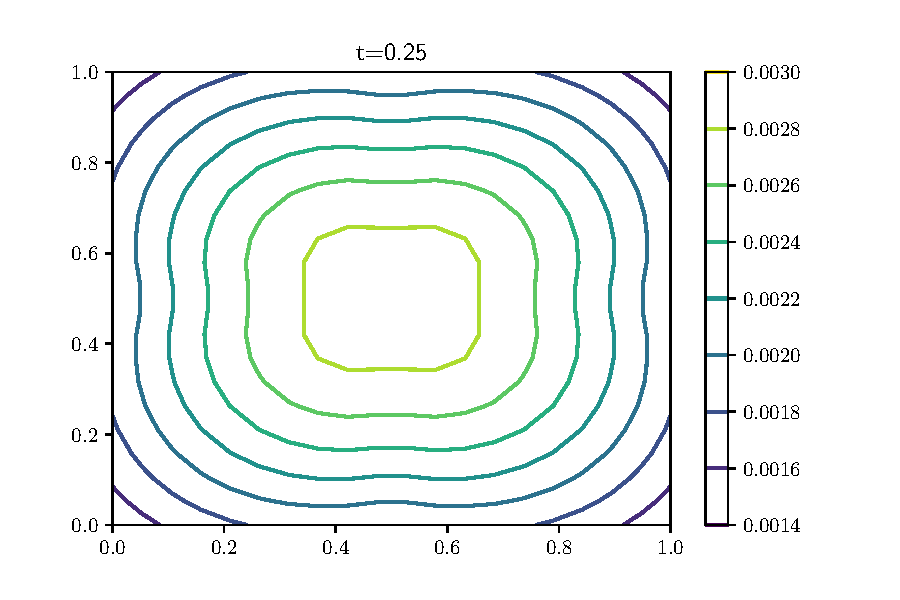
\includegraphics[width=0.8\textwidth]{graphics/rho(1).pdf}
    \caption{rho(t)}
    \label{fig:nu}
\end{figure}
\end{frame}
\begin{frame}{Dynamic formulation: numerical results}
\begin{figure}
    \centering
    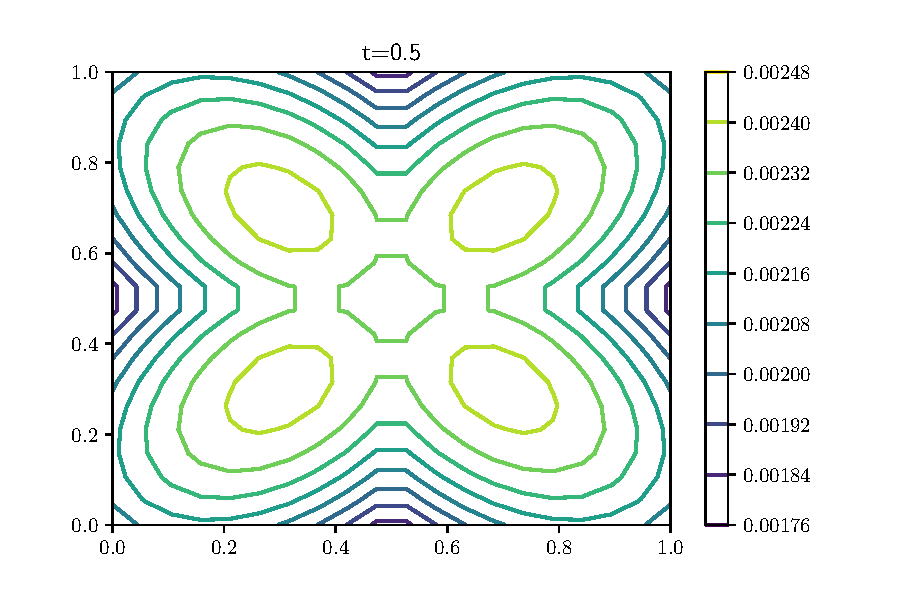
\includegraphics[width=0.8\textwidth]{graphics/rho(2).pdf}
    \caption{rho(t)}
    \label{fig:nu}
\end{figure}
\end{frame}
\begin{frame}{Dynamic formulation: numerical results}
\begin{figure}
    \centering
    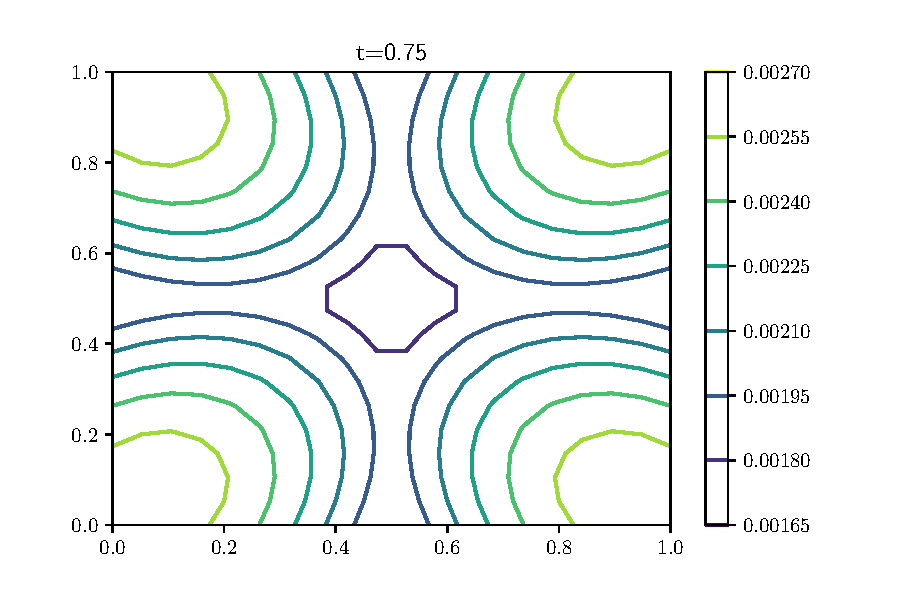
\includegraphics[width=0.8\textwidth]{graphics/rho(3).pdf}
    \caption{rho(t)}
    \label{fig:nu}
\end{figure}
\end{frame}
\begin{frame}{Dynamic formulation: numerical results}
\begin{figure}
    \centering
    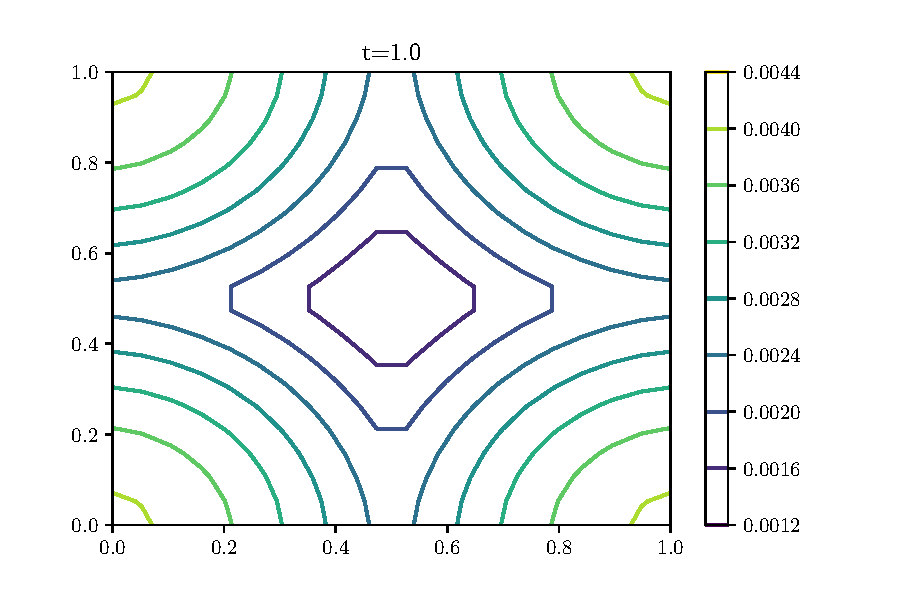
\includegraphics[width=0.8\textwidth]{graphics/rho(4).pdf}
    \caption{rho(t)}
    \label{fig:nu}
\end{figure}
\end{frame}


\begin{frame}{Plan for the next month (4 weeks)}
\begin{itemize}
    \item Implementation the last algorithm (week 1-2, need to hurry up a bit)
    \item Individual tests (weeks 2-3):
    \begin{itemize}
        \item Test on known problems: Gaussian, uniform distributions (compare smooth vs non-smooth).
        \item Check the theoretical complexity by plotting running time with respect to the discretization number.
    \end{itemize}
    \item Comparison tests(weeks 3-4):
    \begin{itemize}
        \item compare their running time
        \item compare the quality of transport
        \item use it on data?
    \end{itemize}
    \item Tries of modifications (if time):
    \begin{itemize}
        \item Hungarian algorithm: Change the indexation, choose a geometric heuristic to sort samples and see if the runtime changes.
        \item Benamou-Brenier: Same stiffness matrix at every Poisson step, try to store its sparse factorization (should be already used by the sparse solver anyway), and use it at each step. If the factorization was really sparse (linear filling), we would get $O(n^2)$ one time to factorize, and  $O(n)$ at each iteration. (but lot of filling in 3D)
        \end{itemize}
\end{itemize}
\end{frame}

\end{document}